\section{IR-analyse af stofferne paracetamol, ibuprofen og R-limonen}\label{IRSPEK}
Vi vil i dette afsnit se nærmere på hvordan man i praksis bestemmer hvilket stof et bestemt IR-spektrum hører til. Der vil ses på de tre stoffer: paracetamol, som blandt andet er det aktive stof i det smertestillende middel panodil , ibuprofen, der også er smertestillende og til sidst stoffet R-limonen, som er en farveløs væske der ved stuetemperatur dufter kraftigt af appelsin.\refLimo     \\
Der er tre forskellige stoffer, som skal tildeles tre forskellige IR-spektre. Man kan indledningsvist se på molekylernes opbygning og gøre det klart for sig selv, ved hvilke bølgelængder man forventer at se absorption. 
\\

Der kigges da på de funktionelle grupper som de tre stoffer indeholder. (Alle de karakteristiske bølgetal for absorptionsbåndene er taget fra BASISKEMI A)\refKemiA{248-249}

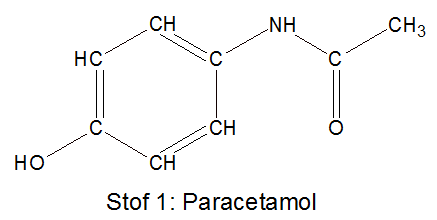
\includegraphics[scale=0.5]{Billeder/paracetamol}
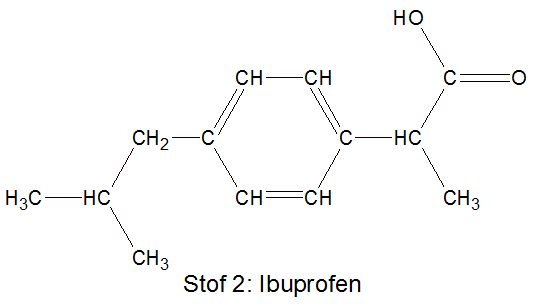
\includegraphics[scale=0.5]{Billeder/ibuprofen}
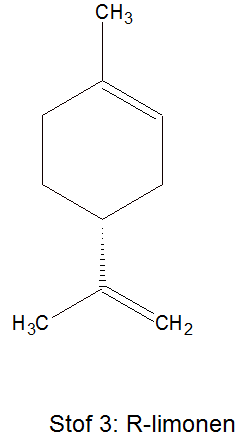
\includegraphics[scale=0.5]{Billeder/Rlimonen}
\vspace{0.8cm}
\begin{enumerate}
\item[\textbf{Stof 1}] 
Stof 1 er paracetamol. De karakteristiske bølgetal for funktionelle grupper vi har tænkt at at kigge efter, når vi skal slå op i vores tabel for bølgetal er følgende: 
\begin{itemize}
\item OH-Ar Fenol, da vi har en alkoholgruppe, som sidder på en aromatisk ring. (\={v}= 3550-3200)

\item N-H: sekundær amid, da vi har en carbonylgruppe, som er bundet til et nitrogenatom, der kun er bundet til 1 hydrogenatom. (\={v}= 3400-3500 og ~1650)

\item CH: $sp^2$-stræk fra den aromatiske ring (\={v}=3010-3100 )

\item C=O: Amidgruppen giver udslag i området (\={v}= 1600-1700)

\item C-H $sp^3$-stræk i området (\={v}= 2810-2960)
\end{itemize}

\item[\textbf{Stof 2}]
Stof 2 er Ibuprofen. Vi er igen interesserede i de karakteristiske bølgetal for de funktionelle grupper som stoffet indeholder. De skrives op i tabellen nedenfor. 

\begin{itemize}
\item C-H: $sp^3$-stræk i området (\={v}= 2810-2960)

\item CH: $sp^2$-stræk i intervallet (\={v}= 3010-3100) for den aromatiske ring. 

\item C=O: Carboxylsyregruppen i ibuprofen giver udslag i området om (\={v}= 1695)

\item O-H: Hydroxylgruppen i ibuprofen giver udslag i området (\={v}= 3000-2500) og er et meget bredt bånd. 
\end{itemize}
\item[\textbf{Stof 3}]
De karakteristiske bølgetal for de funktionelle grupper i R-limonen skrives op

\item H-C=: Bindingen mellem hydrogenatomet og carbonatomet, der sidder i en dobbeltbinding med et andet carbonatom giver udslag i området (\={v}=  3010-3100)

\item C-H $sp^3$: giver udslag i området (\={v}= 2810-2960)

\item C=C $sp^2$: Giver udslag i området (\={v}= 1600-1700)
\end{enumerate}

De tre stoffer skal nu knyttes til hver deres IR-spektrogram se bilag 4, 5 og 6. For at overskueliggøre denne process, tager vi udgangspunkt i forskellene på de funktionelle grupper som de tre stoffer indeholder. R-limonen indeholder for eksempel ikke nogen hydroxylgruppe og vil ikke have det kendetegnende brede \emph{tungebånd} i området omkring (\={v} $\approx$ 3000). Hvis vi kigger på bilagene med de tre IR-spektre kan vi se, at dette udelukker både bilag 4 og 5. Vi kan altså næsten øjeblikkeligt slutte, at stoffet R-limonen hører til det IR-spektrum på bilag 6. Det undersøges lidt nærmere for en sikkerheds skyld. 
\\

Hvis bilag 6 skulle være det IR-spektrum af R-limonen skulle vi se absorbtionsbånd for de funktionelle grupper der er i R-limonen. Dette indebærer et et udslag i området (\={v}= 1600-1700) - Dette kan vi bekræfte at der også er på bilag 6, et udslag i området (\={v}= 2810-2960) - dette er også tilstedeværende på vores IR-spektrummet, og et udslag ved (\={v}= 3010-3100) som formegentligt er blevet forskudt lidt mod højre og flyder ind i nabobåndet. 
\\

Alt taget i betragtning virker bilag 6 til at være et godt bud på, at være et IR-spektrum af R-limonen.
\\

Nu betragtes de to resterende stoffer og deres IR-spektre. Én af de funktionelle grupper, der adskiller de to stoffer er paracetamols sekundære amid, som gav udslag i området omkring (\={v} $\approx$ 1650). Kigger vi på de to spektre på hhv. bilag 4 og 5 vil vi se, at der kun optræder et absorptionsbånd omkring (\={v} $\approx$ 1650) på bilag 4. Det absorptionsbånd som kommer tættest på, er absorptionsbåndet der ligger omkring de \={v} $\approx$ 1700, men dette absorptionsbånd kan tildeles til C=O strækket for carbonylgruppen i ibuprofen.
\\

Vi kan yderligere bekræfte formodningen om at det IR-spektrum på bilag 4 hører til stof 1 og at IR-spektrummet på bilag 5 hører til stof 2.
\\

Dette kan også verificeres ved at se på OH-gruppen i begge stoffer. Da hydroxylgruppen i stof 1 sidder på en aromatisk ring vil den give udslag ved et højere bølgetal end, hvis den havde siddet som en del af en carboxylsyre, som er tilfældet i stof 2. Dette kan vi også se, hvis vi betragter de to spektre. På spektret på bilag 4 har vi et tungebånd med centrum i omkring (\={v}= 3200) og på spektret på bilag 5 har vi et tungebånd med centrum omkring (\={v}= 2750).
\\

Dette gør det muligt for at tildele de tre spektre til de tre stoffer. Stof 1 (Paracetamol) hører til IR-spektret på bilag 4, stof 2 (Ibuprofen) hører til IR-spektret på bilag 5 og stof 3 (R-limonen) hører til IR-spektret på bilag 6.